%!TEX TS-program = pdflatex
%!TEX TS-options = -shell-escape
% Author: Phil Steinhorst, p.st@wwu.de
% https://github.com/phist91/latex-templates

\newcommand{\obenlinks}{Recurrent and Generative Artificial Neural Networks}
% Author: Phil Steinhorst, p.st@wwu.de
% https://github.com/phist91/latex-templates

\documentclass[%
	paper=a4,
	fontsize=10pt,
	english
	]{scrartcl}

% Basics für Codierung und Sprache
% ===========================================================
	\usepackage{scrtime}
	\usepackage{etex}
	\usepackage{shellesc}					% Compiler-Option -shell-escape benutzen!
	\usepackage[final]{graphicx}			% Einbindung von Grafiken
	\usepackage[utf8]{inputenc}				% Dateien sind UTF8-codiert
	\usepackage{babel}						% deutsche Silbentrennung, etc.
	\usepackage[]{csquotes}	% deutsche Anführungszeichen mit \enquote{...}
% ===========================================================

% Fonts und Typographie
% ===========================================================
	\usepackage{sourcecodepro}
	\usepackage[default]{sourcesanspro}
	\usepackage{nimbusmononarrow}
	
	\usepackage[babel=true,final,tracking=smallcaps]{microtype}
	\DisableLigatures{encoding = T1, family = tt* } % keine Ligaturen für Monospace-Fonts
	\usepackage{ellipsis}
% ===========================================================

% Farben
% ===========================================================
	\usepackage[usenames,x11names,final]{xcolor}
% ===========================================================

% Mathe-Pakete und -Einstellungen
% ===========================================================
	\usepackage{mathtools}					% Tools zum Setzen von Formeln
	\usepackage{amssymb}					% übliche Mathe-Symbole
	\usepackage[bigdelims]{newtxmath}		% moderne Mathe-Font
	\allowdisplaybreaks						% seitenübergreifende Rechnungen
	\usepackage{bm}							% math bold font
	\usepackage{bbm}
	\usepackage{wasysym}					% noch mehr Symbole
% ===========================================================

% TikZ
% ===========================================================
	\usepackage{tikz}
	\usepackage{tikz-cd}					% kommutative Diagramme
	\usetikzlibrary{arrows.meta}			% mehr Pfeile!
	\usetikzlibrary{calc}					% TikZ kann rechnen
	\tikzset{>=Latex}						% Standard-Pfeilspitze
% ===========================================================

% Seitenlayout, Kopf-/Fußzeile
% ===========================================================
	\usepackage{scrpage2}
	\pagestyle{scrheadings}
	\usepackage[top=3cm, bottom=3cm, left=2.5cm, right=2cm]{geometry}
	\clearscrheadfoot 
	\setheadsepline{0.4pt}			 					% Linie in Kopfzeile
	\setfootsepline{0.4pt}								% Linie in Fußzeile
	\setkomafont{pagehead}{\bfseries}					% Schriftart Kopfzeile
	\setkomafont{pagefoot}{\normalfont\footnotesize}	% Schriftart Fußzeile 
	\cfoot{\thepage}									% Seitenzahl unten Mitte
	\lohead{\obenlinks}	% Titel oben links
	\raggedbottom							% Flattersatz
	\usepackage{setspace}					% erweiterte Abstandsoptionen
	\onehalfspacing							% Zeilenabstand 1.5-fach
	\setlength{\parindent}{0pt}				% Einrückung neuer Absätze
	\setlength{\parskip}{0.5\baselineskip}	% Abstand neuer Absätze
% ===========================================================

% Hyperref für Referenzen und Hyperlinks
% ===========================================================
	\usepackage[%
		hidelinks,
		pdfpagelabels,
		bookmarksopen=true,
		bookmarksnumbered=true,
		linkcolor=black,
		urlcolor=SkyBlue2,
		plainpages=false,
		pagebackref,
		citecolor=black,
		hypertexnames=true,
		pdfborderstyle={/S/U},
		linkbordercolor=SkyBlue2,
		colorlinks=false,
		backref=false]{hyperref}
	\hypersetup{final}
% ===========================================================

% Listen und Tabellen
% ===========================================================
	\usepackage{multicol}
	\usepackage[shortlabels]{enumitem}
	\setlist{itemsep=0pt}
	\setlist[enumerate]{font=\sffamily\bfseries}
	\setlist[itemize]{label=$\triangleright$}
	\usepackage{tabularx}
% ===========================================================

% minted
% ===========================================================
\usepackage{minted}
\setminted{%
	style=default,
	fontsize=\small,
	breaklines,
	breakanywhere=false,
	breakbytoken=false,
	breakbytokenanywhere=false,
	breakafter={.,},
	autogobble,
	numbersep=3mm,
	tabsize=4,
	linenos,
	frame=lines
}
\setmintedinline{%
	fontsize=\normalsize,
	numbers=none,
	numbersep=12pt,
	tabsize=4,
}

% Weitere Importe
% ===========================================================
\usepackage{todonotes}
% ===========================================================


%%%%%%%%%%%%%%%%%%%%%%%%%%%%%%%%%%%%%%%%%%%%%%%%%%%%%%%%%%%
%%% Ab hier folgen nur noch vordefinierte Mathe-Befehle %%%
%%%%%%%%%%%%%%%%%%%%%%%%%%%%%%%%%%%%%%%%%%%%%%%%%%%%%%%%%%%

\newcommand{\BB}{\mathbb{B}}
\newcommand{\CC}{\mathbb{C}}
\newcommand{\NN}{\mathbb{N}}
\newcommand{\QQ}{\mathbb{Q}}
\newcommand{\RR}{\mathbb{R}}
\newcommand{\ZZ}{\mathbb{Z}}
\newcommand{\oh}{\mathcal{O}}						
\newcommand{\ol}[1]{\overline{#1}}
\newcommand{\wt}[1]{\widetilde{#1}}
\newcommand{\wh}[1]{\widehat{#1}}

\DeclareMathOperator{\id}{id} 				% Identität
\DeclareMathOperator{\pot}{\mathcal{P}}		% Potenzmenge

% Klammerungen und ähnliches
\DeclarePairedDelimiter{\absolut}{\lvert}{\rvert}		% Betrag
\DeclarePairedDelimiter{\ceiling}{\lceil}{\rceil}		% aufrunden
\DeclarePairedDelimiter{\Floor}{\lfloor}{\rfloor}		% aufrunden
\DeclarePairedDelimiter{\Norm}{\lVert}{\rVert}			% Norm
\DeclarePairedDelimiter{\sprod}{\langle}{\rangle}		% spitze Klammern
\DeclarePairedDelimiter{\enbrace}{(}{)}					% runde Klammern
\DeclarePairedDelimiter{\benbrace}{\lbrack}{\rbrack}	% eckige Klammern
\DeclarePairedDelimiter{\penbrace}{\{}{\}}				% geschweifte Klammern
\newcommand{\Underbrace}[2]{{\underbrace{#1}_{#2}}} 	% bessere Unterklammerungen
% Kurzschreibweisen für Faule und Code-Vervollständigung
\newcommand{\abs}[1]{\absolut*{#1}}
\newcommand{\ceil}[1]{\ceiling*{#1}}
\newcommand{\flo}[1]{\Floor*{#1}}
\newcommand{\no}[1]{\Norm*{#1}}
\newcommand{\sk}[1]{\sprod*{#1}}
\newcommand{\enb}[1]{\enbrace*{#1}}
\newcommand{\penb}[1]{\penbrace*{#1}}
\newcommand{\benb}[1]{\benbrace*{#1}}
\newcommand{\stack}[2]{\makebox[1cm][c]{$\stackrel{#1}{#2}$}}	% Präambel (ohne die geht nichts!)
\begin{document}
\begin{center}
	\begin{tabular}{|rlp{4cm}rl|}
	\hline
	 \textbf{Exercise Sheet} & 02  &  & \textbf{1. Team Partner:} & Lennart Slusny  \\
	 \textbf{Task} & 01 & & \textbf{2. Team Partner:} & Joschka Strüber \\ \hline
	\end{tabular}
\end{center} 

\textbf{(a)} How can LSTMs and other gated memory units learn to count and solve other discrete tasks? What is expected to happen during training?

\textbf{Answer:} 

The time steps of an RNN act as a natural source of discreteness. However, because of the aforementioned smooth and continuous functions make sharp calculations in ungated RNNs very difficult to learn.

Here comes the gates and especially the forget gate into play. The cell state $s^t_c$ is computed as the input gate activation times the squashed cell input added to the forget gate multiplied with the previous cell state:

\begin{equation}
	s_c^t = x_l^t \odot g_c(\operatorname{net}_c^t) + x_{\phi}^t \odot s_c^{t-1}
\end{equation}

While the sigmoid activation function for the gates is smooth and continuous in theory, in practice the sigmoid saturates very quickly to almost 0 for small inputs and almost 1 for large inputs. As a result, the cell state is very often not a truly continuous mixture between inputs and recurrences, but rather the switches turn completely on or off. This drastic behavior of the gates allows to learn sharp and pretty much discrete function.

This effect is also very beneficial for training these networks and allows to effectively learn much longer dependencies. Whenever the values of the forget gate are almost 1, the gradients backpropagating through time from $\nabla_{\theta} s_c^t$ to $\nabla_{\theta} s_c^{t-1}$ remain the same. Once the gate is turned off and its values are close to zero, the corresponding gradient is cut off between time steps.

\textbf{(b)} Consider a single LSTM unit with D memory cells. Starting with 

\begin{equation}
	\delta_\phi^t = \frac{\partial E}{\partial \operatorname{net}_\phi^t}
\end{equation}

derive the forget gate gradient of the LSTM:

\begin{equation}
	\delta_\phi^t = \varphi'_\phi(\operatorname{net}_\phi^t) \sum_{c=1}^{D} \zeta_c^t s_c^{t-1}
\end{equation}

\textbf{Answer:} 

\begin{align}
	\delta_\phi^t &= \frac{\partial E}{\partial \operatorname{net}_\phi^t} \\
	&= \frac{\partial x_\phi^t}{\partial \operatorname{net}_\phi^t} \frac{\partial E}{\partial x_\phi^t} \\
	&= \frac{\partial \varphi_\phi(\operatorname{net}_\phi^t)}{\partial \operatorname{net}_\phi^t} \frac{\partial E}{\partial x_\phi^t} \\
	&= \varphi_\phi'(\operatorname{net}_\phi^t) \frac{\partial E}{\partial x_\phi^t} \\
\end{align}

This way, we derived the first part of the forget gate gradient. Next, we focus on the second part. The forget gate is used to compute the cell state for every of the $D$ cells by element-wise multiplication. Hence, we have to consider the gradient for the vector of internal states at time step $t$:

\begin{align}
	\delta_\phi^t &= \varphi_\phi'(\operatorname{net}_\phi^t) \frac{\partial E}{\partial x_\phi^t} \\
	&=  \varphi_\phi'(\operatorname{net}_\phi^t) (\nabla_{x_{\phi}^t} s^t)^T \nabla_{s^t} E \\
	&=  \varphi_\phi'(\operatorname{net}_\phi^t) \sum_{c \in D} \frac{\partial s_c^t}{\partial x_{\phi}^t} \frac{\partial E}{\partial s_c^t} \\
	&=  \varphi_\phi'(\operatorname{net}_\phi^t) \sum_{c \in D} \frac{\partial \left(x_l^t g_c(\operatorname{net}_c^t) + x_\phi^t s_c^{t-1}\right)}{\partial x_{\phi}^t} \zeta_c^t \\
	&=  \varphi_\phi'(\operatorname{net}_\phi^t) \sum_{c \in D} s_c^{t-1} \zeta_c^t
\end{align}

\textbf{(c)} Can bidirectional RNNs be effectively used for online classification, that is generating a classification label for every new input immediately? Explain briefly.

\textbf{Answer:} No, that is in general not possible. To make inference, a bidirectional RNN needs both pretemporal and posttemporal context to compute an output. However, in  online classification, only the pretemporal context is available. To get the posttemporal context, we would have to get to the end of a timeseries and compute the recurrence back in time, which is impossible in this context.


\begin{center}
	\begin{tabular}{|rlp{11cm}|}
		\hline
		\textbf{Task} & 02 & \\ \hline
	\end{tabular}
\end{center} 

\textbf{(a)} Name three forms of commonly applied regularization techniques for neural networks and describe their effects.

\textbf{Answer:}

Early stopping uses a separate evaluation set to monitor the error of the model. At one point, the model will very likely stop to generalize well and start to overfit on the training set. Since we monitor the error on the validation set, that is not used for training, we can very likely find this moment of the training process, stop the training and return the model that performed best on the validation set. Because it is assumed to come from the same distribution as the test set, we expect the returned model to be the best of that training regime on the test set as well.

Weight decay adds a regularization term based on the model's weight to the error:

\begin{equation}
	\hat{E}(\mathbf{w}) = E(\mathbf{w}) + \lambda \Omega(\mathbf{w})
\end{equation}

$\Omega$ can be any metric that punishes large weights, e.g. the Manhattan or Euclidean distance. Since the regularization is part of the loss, we also calculate the gradient with respect to the regularization that is used for updating the weights:

\begin{equation}
	w_i \leftarrow w_i + \eta \frac{\partial E(\mathbf{w})}{\partial w_i} + \eta \lambda \frac{\partial E(\mathbf{w})}{\partial w_i}
\end{equation}

In other words, the weights are decreased or \enquote{decay} in each training step based on their size, hence the method's name.

Deep neural network tend to produce sharp, low-entropy, over-confident results by memorizing the training data. To counteract this effect, label smoothing adds noise to the training labels, by decreasing the values of positive classes and increase those of negative classes in one-hot vectors. Given a single-label classification problem with $N$ classes, we choose a small $\epsilon$ as hyper parameter and modify the labels $y$ as follows:

\begin{align}
	\hat{y}_i &= \frac{\epsilon}{N-1} &\text{, if } y_i = 0 \\
 	\hat{y}_i &= 1 - \epsilon & \text{, if } y_i = 1
 \end{align}

\textbf{(b)} Explain the internal covariate shift and how it has been addressed in the literature.

\textbf{Answer:}

Given a layer, when the parameters of the previous layer change, so does the statistics of the current's inputs. Therefore, the current layer has to adjust to changing targets during the training process and becomes instable, if the learning rates are too large or the weight initialization is chosen unfavorably. 

This problem is addressed by batch normalization. This technique computes the mean and variance of each mini-batch and uses them to normalize a layer's input. This way, the input always has comparable statistics. Apart of the normalization, the input is also scaled and shifted by two learnable parameters $\gamma$ and $\beta$. 

At the test phase, the learnable parameters are frozen and the normalizing mean and variance parameters are computed over the whole data set as a moving average, to get a deterministic inference that works well for the whole training data set.

\textbf{(c)} Consider the following statement: The more parameters a neural network has the better it will generalize. Is this statement true?

\textbf{Answer:}

In general, a model with more parameters has a higher chance of learning more complex functions and has the ability to generalize well. However, in practice there is a higher chance of overfitting to the seen training data, which hampers the model's ability to generalize. This corresponds to the classical regime of learning theory with a training risk that decreases with increasing model capacity - and hence number of parameters in our case - and increasing test risk, if the model capacity becomes too large. 

However, \cite{belkin19} have shown that the test error start decreasing again for models with a very large model capacity, eg. deep neural networks with millions of parameters. Cf. the visualization in figure \ref{img:double-descent}. The left-hand side shows the classic bias-variance tradeoff, where the model start overfitting if the capacity becomes too large. The right side shows the double-descent risk-curve, where the test error suddenly starts decreasing again for even larger model capacities.

\begin{figure}
	\begin{center}
		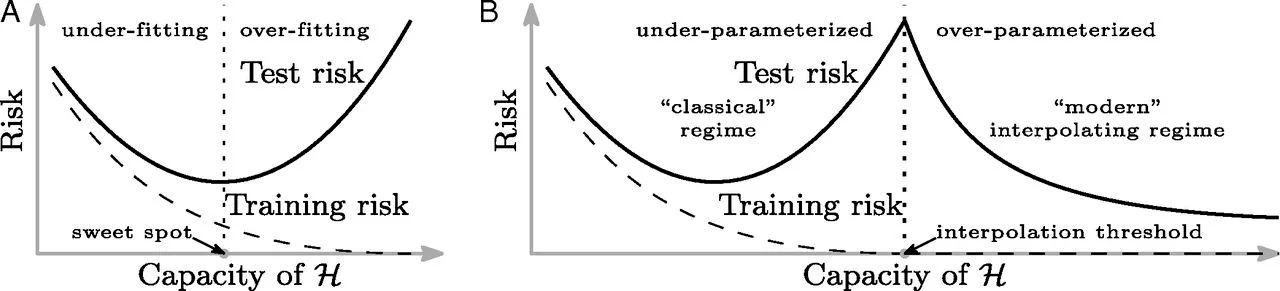
\includegraphics[width=0.8\linewidth]{belkin19}
		\caption{Curves for the training and test risk in the classical and modern regime of learning theory \cite{belkin19}.}
		\label{img:double-descent}
	\end{center}
\end{figure}

\textbf{(d)} What is the effect of residual blocks on the gradient flow in deep networks?

\textbf{Answer:}

Residual nets use shortcuts to take a layers output as identity and add them as an additional output by skipping a block of weight layers. This way, the function learned inside the residual block that was skipped can be seen as learning the offset from the identity. 

Given a net activation $x_l$, a net activation $x_L$ further down in the computation graph and weights functions $f_i$ for the intermediate blocks that were skipped with residual connections, $x_L$ can be computed based on $x_l$ in the following way:

\begin{equation}
	x_L = x_l + \sum_{i=l}^{L-1} f_i(x_i) 
\end{equation}

This makes sense, because the output after each residual block is added to the identity that is propagated via skip connections, but also further processed by the next residual blocks. 

As a result, the gradient also backpropagates nicely as the identity, because of the skip connections, and it is modified additively based on the gradients of the residual blocks:

\begin{align}
	\frac{\partial E}{\partial x_l} &= \frac{\partial E}{\partial x_L} \frac{\partial x_L}{\partial x_l} \\
	&= \frac{\partial E}{\partial x_L} \left( 1 - \frac{\partial}{\delta x_l} \sum_{i=l}^{L-1} f_i(x_i) \right)
\end{align}

In this way, the gradient is very unlikely to vanish, because of the identity skip connections. This decreases the chance of the vanishing gradient problem significantly and allows to train much deeper networks than before.

\begin{center}
	\begin{tabular}{|rlp{11cm}|}
		\hline
		\textbf{Task} & 03 & \\ \hline
	\end{tabular}
\end{center} 

\textbf{(a)} What is the general purpose of autoencoders (AEs) and what are their main components? Give an illustration.

\textbf{Answer:}

Autoencoders are based on a decoder and an encoder, as can be seen in figure \ref{img:ae}. The encoder maps the input to a lower-dimensional latent space. The decoder tries to reproduce the input based on the latent state by minimizing a reconstruction error, eg. L2.

This model architecture can be used for compressing data, as the latent state is typically of a lower dimensionality, and to generate new data based on sampled instances in the latent space.

\begin{figure}
	\centering
	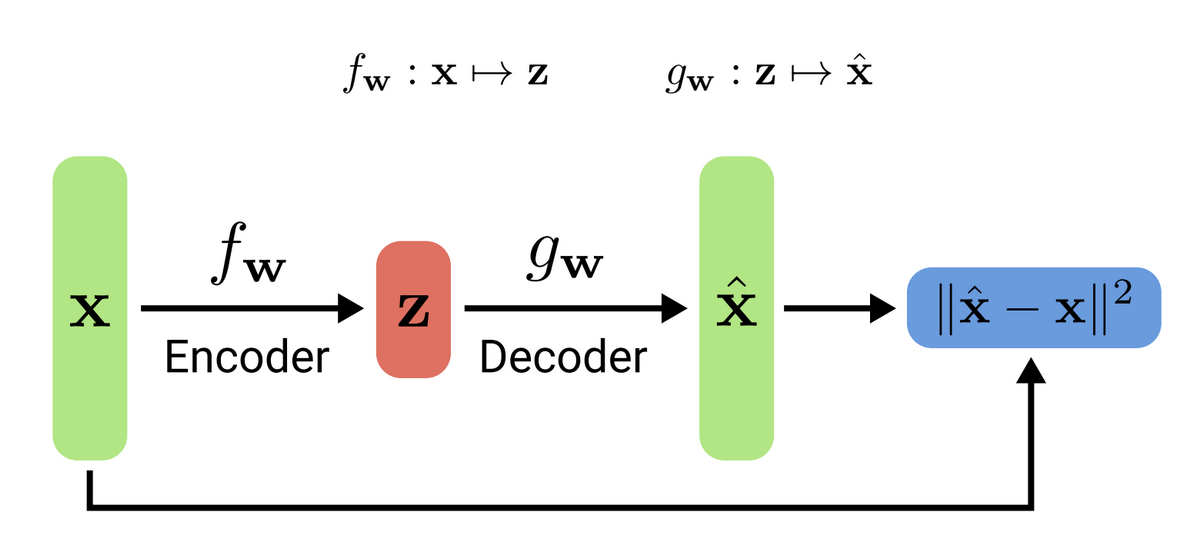
\includegraphics[width=0.8\linewidth]{ae}
	\caption{Visualization of an autoencoder with decoder, latent state and decoder \cite[7 L. 11]{geiger20}}
	\label{img:ae}
\end{figure}

\textbf{(b)} Briefly explain the purpose of the KL divergence.

\textbf{Answer:}

The Kullback-Leibler divergence $\operatorname{KL}$ is a distance function to measure the difference between a probability distribution $P$ to a reference distribution $Q$. It measures the expected additional Shannon-information, if $Q$ is used instead of the true distribution $P$. The KL-divergence is defined as follows:

\begin{equation}
	\operatorname{KL}(P||Q) = \sum_{x \in \Omega} P(x) \log \left( \frac{P(x)}{Q(x)} \right)
\end{equation}

\textbf{(c)} Given two discrete probability distributions $Q, P$. Show that $\operatorname{KL}(Q || P) = \operatorname{KL}(P || Q)$ does not hold in general.

\textbf{Answer:}

We show this by constructing a simple counter example based on two Bernoulli distributions. 

\begin{align}
	P(x) &= \left\{
		\begin{array}{ll}
			0.3 & \text{, if x = 0} \\
			0.7 & \text{, if x = 1}
		\end{array} \right.
	Q(x) &= \left\{
		\begin{array}{ll}
			0.5 & \text{, if x = 0} \\
			0.5 & \text{, if x = 1}
		\end{array} \right.
\end{align}

Now we can compute the KL-divergences in both directions:

\begin{align}
	\operatorname{KL}(P||Q) &= 0.3 \cdot \log_2 \left( \frac{0.3}{0.5}\right) + 0.7 \cdot \log_2 \left( \frac{0.7}{0.5}\right) \\
	& \approx 0.1187 \\
	\operatorname{KL}(Q||P) &= 0.5 \cdot \log_2 \left( \frac{0.5}{0.3}\right) + 0.5 \cdot \log_2 \left( \frac{0.5}{0.7}\right) \\
	& \approx 0.1258
\end{align}

Since $0.1187 \neq 0.1258$, we have shown that the KL-divergence is not symmetric in general.

%- 0.3 * log_2(0.3/0.5) - 0.7 * log_2(0.7/0.5) = -0.1187

%- 0.5 * log_2(0.5/0.3) - 0.5 * log_2(0.5/0.7) = -0.1258

\textbf{(d)} Briefly describe the re-parametrization trick and explain why it is necessary to train a VAE.

\textbf{Answer:}

Variational autoencoders try to minimize the negative log likelihood that is upper bounded using the ELBO. This target function separates into the variational loss and reconstruction loss. The variational loss is the KL-divergence between the distribution of the encoder for the latent state given the data and a prior on the decoder:

\begin{equation}
	\operatorname{KL}(q(\mathbf{h}|\mathbf{x}) || p(\mathbf{x}))
\end{equation}

The deconstruction loss describes how well the decoder is able to reconstruct the input based on the distribution given by the encoder:

\begin{equation}
	- \mathbb{E}_{h\sim q(\mathbf{h}|\mathbf{x})} \log p(\mathbf{x} | \mathbf{h})
\end{equation}

To have a target for the distribution of the encoder, we use a standard Gaussian $N(\mathbf{0}, \mathbf{1})$ as variational prior. We also assume that the encoders learned distribution is a Gaussian $N(\mathbf{\mu}, \mathbf{\sigma})$. This way, the latent code corresponds to just the parameters $\mathbf{\mu}, \mathbf{\sigma}$ that fully describe the distribution and the variational loss separates into a nice and simple formula:

\begin{equation}
	\operatorname{KL}(N(\mathbf{\mu}, \mathbf{\sigma})|| N(\mathbf{0}, \mathbf{I}) = \frac{1}{2} e^{\sigma^2} + \mathbf{\mu}^2 - 1 - \sigma^2
\end{equation}

This formula is fully differential, which makes training easy. For a forward pass, we can simply sample from $N(\mathbf{0}, \mathbf{1})$ and modify them with the current latent space parameters to generate a new latent code:

\begin{equation}
	\mathbf{h}(\mathbf{x}) = \mu(\mathbf{x}) + \sigma(\mathbf{x}) \cdot N(\mathbf{0}, \mathbf{1})
\end{equation}

Finally, the reparametrization trick is to treat the samples as constant factors, which allows to train both encoder and decoder via backpropagation. This step is important, because in the original formulation, we sample latent states inside the network directly from $N(\mathbf{\mu}, \mathbf{\sigma})$, which is intractable.

\textbf{(e)} Name a frequently mentioned drawback of VAEs and give one example from the literature that addresses this issue.

\textbf{Answer:}

The main drawback of original VAEs compared to eg. GANs was that the generated images tend to be not a sharp, but slightly blurry. This was addressed by further improvements, such as the Vector-Quantized Variational Autoencoder (VQ-VAE 2) \cite{razavi19}. This method uses prototype vectors from a learned codebook in the latent space and samples from an autoregressive model. As a result, its generated images are much sharper and come close to the SOTA of GANs.

\textbf{(f)} What are the major differences of the variational autoencoders (VAEs) in comparison with standard autoencoders? Relate your answer to the two sub-losses that are optimized during VAE training.

\textbf{Answer:}

Autoencoders only use a reconstruction loss to minimize the difference between original inputs and decodings. VAEs, on the other hand, aim to minimize the negative log likelihood, which can be upper bounded via the ELBO into the original reconstruction loss and a variational loss that minimizes the difference between the model's distribution and a variational prior distribution.

Since this prior was chosen as $N(\mathbf{0}, \mathbf{1})$, we push the distribution of latent codes to be roughly standard Gaussian. This allows us to treat the VAEs as probabilistic generator of a data distribution and we can generate new data by simply sampling random noise from a standard Gaussian and pass them to the predicted distribution parameters to generate new latent codes. 

\textbf{(g) Bonus:} Show that the $\operatorname{KL}$-divergence between two Gaussian distributions simplifies in the following form, if the reference distribution is the standard normal:

\begin{equation}
	\operatorname{KL}(N(\mathbf{\mu}, \mathbf{\Sigma})|| N(\mathbf{0}, \mathbf{I}) = \frac{1}{2} \sum_{i=1}^k \left(\sigma_i^2 + \mu_i^2 - 1 - \log(\sigma_i^2) \right)
\end{equation}

\textbf{Answer: } We are given the general form of the KL-divergence:

\begin{equation}
	\operatorname{KL}(N(\mathbf{\mu_1}, \mathbf{\Sigma_1})||N(\mathbf{\mu_2}, \mathbf{\Sigma_2}))  = \frac{1}{2} \left\{ \operatorname{tr}(\Sigma_2^{-1}  \Sigma_1) + (\mathbf{\mu_2} - \mathbf{\mu_1})^T \Sigma_2^{-1} (\mathbf{\mu_2} - \mathbf{\mu_1}) - k - \log \frac{\det \Sigma_2}{\det \Sigma_1} \right\}
\end{equation}

Plugging in $N(\mathbf{\mu}, \mathbf{\Sigma})$ and $N(\mathbf{0}, \mathbf{I}$, this yields:

\begin{align}
	\operatorname{KL}(N(\mathbf{\mu}, \mathbf{\Sigma})|| N(\mathbf{0}, \mathbf{I}) &= \frac{1}{2} \left\{ \operatorname{tr}(\mathbf{I}^{-1}  \Sigma) + (- \mathbf{\mu})^T \mathbf{I}^{-1} (- \mathbf{\mu}) - k + \log \frac{\det \mathbf{I}}{\det \Sigma} \right\} \\
	&= \frac{1}{2} \left\{ \operatorname{tr}(\Sigma) + \mathbf{\mu}^T \mathbf{\mu} - k - \log( \det \Sigma) \right\}
\end{align}

Since, the covariance is a diagonal matrix $\Sigma = \operatorname{diag}(\sigma_1^2, \dots \sigma_k^2)$, the trace and log determinant simplify in the following way:

\begin{align}
	\operatorname{tr}(\Sigma) &= \sum_{i=1}^k \sigma_i^2 \\
	\mathbf{\mu}^T \mathbf{\mu} &= \sum_{i=1}^k \mathbf{\mu}_i^2 \\
	\det \Sigma &= \prod_{i=1}^k \sigma_i^2 \\
	\Rightarrow \log( \det \Sigma) &= \log \prod_{i=1}^k \sigma_i^2 \\
	&= \sum_{i=1}^k \log \sigma_i^2
\end{align}

By plugging them into the previous formula, we get:

\begin{align}
	\operatorname{KL}(N(\mathbf{\mu}, \mathbf{\Sigma})|| N(\mathbf{0}, \mathbf{I}) &= \frac{1}{2} \left\{ \operatorname{tr}(\Sigma) + \mathbf{\mu}^T \mathbf{\mu} - k - \log( \det \Sigma) \right\} \\
	&= \frac{1}{2} \left\{ \sum_{i=1}^k \sigma_i^2 + \sum_{i=1}^k \mathbf{\mu}_i^2 - \sum_{i=1}^k 1 - \sum_{i=1}^k \log \sigma_i^2 \right\} \\
	&=  \frac{1}{2} \left\{ \sum_{i=1}^k \left( \sigma_i^2 + \mathbf{\mu}_i^2 - 1 - \log \sigma_i^2 \right) \right\} 
\end{align}


\begin{center}
	\begin{tabular}{|rlp{11cm}|}
		\hline
		\textbf{Task} & 03 & \\ \hline
	\end{tabular}
\end{center} 

\textbf{(a)} Illustrate the major structure of GANs and name the essential components. Briefly describe the principle. 

\textbf{Answer:}

\begin{figure}
	\centering
	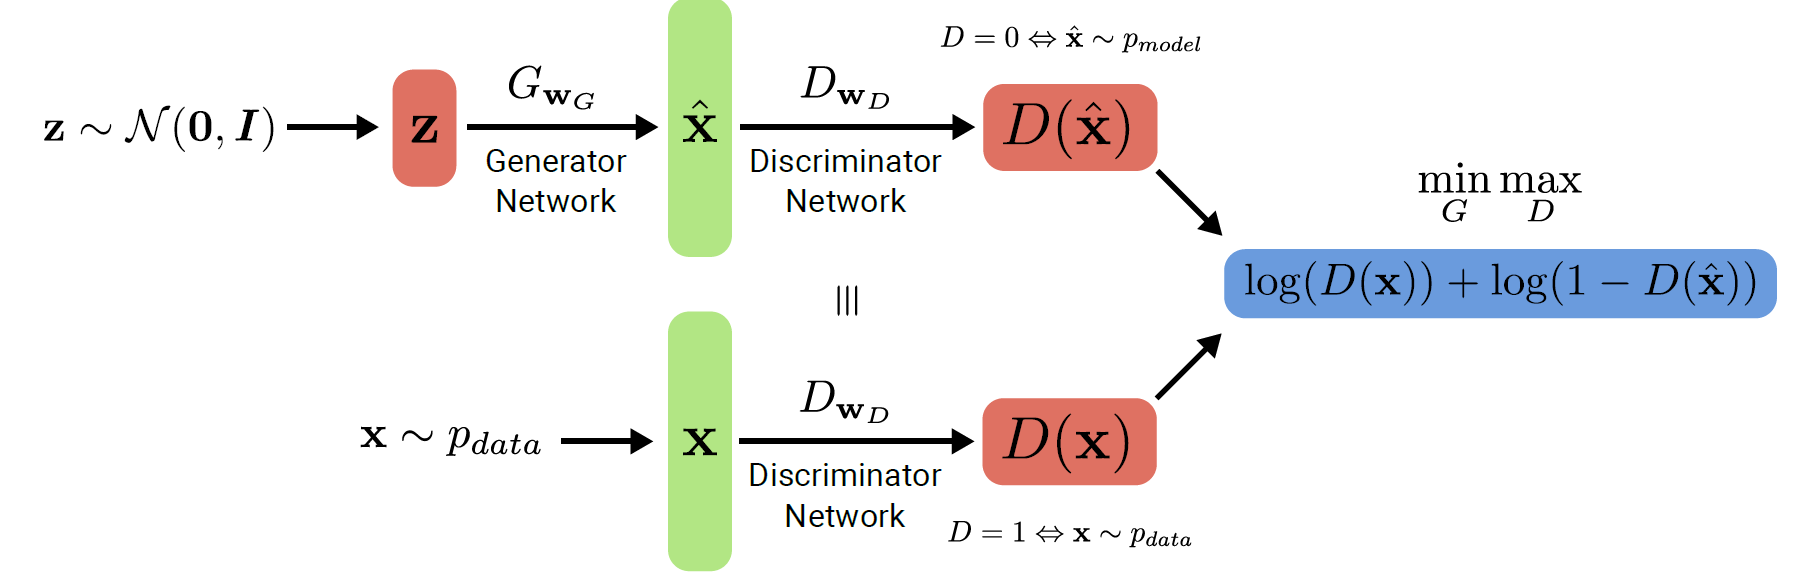
\includegraphics[width=0.8\linewidth]{gan}
	\caption{A Generative Adversarial Network (GAN) with generator G and discriminator D \cite[10, L. 12]{geiger20}.}
	\label{img:gan}
\end{figure}

Just like VAEs, GANs are based on two major components: the generator and the discriminator. The generators goal is to generate data that is as similar as possible to the original training data. The discriminator has to distinguish between real data from the training data set and artificial data generated by the generator. The general structure of a GAN can be seen in figure \ref{img:gan}.

If everything works out perfectly, both networks are about equally capable and improve each other over time: to fool the discriminator, the generator learns to generate more realistic artificial data. Since the generated data is getting more realistic, the discriminator has to become better and recognizing fake data. In practice, this is not as easy and GANs tend to be very hard to train, as described in the next task.


\textbf{(b)} Elaborate on why the training of GANs is considered as particularly difficult/challenging and how it is addressed. Comment on what happens if the discriminator dominates the generator and vice versa.

\textbf{Answer:}

The training process of GANs involves the joint optimization of two different neural networks two-player minimax game. The training process only works efficiently, if both networks are about equally good, because the respective training objectives should be difficult, to enforce learning, but not impossible.

If the discriminator dominates the generator, the generator cannot learn how to generate data that fools the discriminator, because the discriminator is to good at distinguishing. If the generator dominates the discriminator, the latter is not able to discriminate between real training and generated data. As a result, the training objective for the generator is far too easy and it has no incentive to generate more realistic data.

These two problems are addressed in several ways: first of all, there is an alternating optimization scheme that optimizes the discriminator for a fixed sets of steps $k$ and afterwards the generator for a single step. This ensures the discriminator $D$ is always close to its optimal solution, because the generator $G$ does not change too quickly. 

Especially at the beginning, when the generated data is very unrealistic, the discriminator tends to reject artificial samples with high confidence. As a result, the generator objective $\log(1 - D(G(\mathbf{z}))$ saturates, its gradient is very small and the training very slow. This is addressed with the gradient trick by replacing $\log(1 - D(G(\mathbf{z}))$ with $-\log(D(G(\mathbf{z}))$ in the beginning of the training. This function has the same target and direction of the gradient, but the gradient is much larger for small inputs. Later, we can switch back to the original target function, when its gradient becomes better.

\printbibliography

\end{document}